\section{A Matheuristic for the Mothership-Drone Routing Problem with Graphs}\label{Math}
\noindent
This section is devoted to present our matheuristic approach to address the solution of the \AMD. Our motivation comes from the fact that the exact solution of the models presented in Section \ref{Form} is highly time demanding. Alternatively, the matheuristic provides good quality solution in limited computing times.\\
\noindent
%\JP{First, we focus on the synchronized case in which each drone that is used must be launched and retrieved in the same stage.}
The basic idea of the algorithm is to determine the route that a drone should perform for visiting each graph $g \in \mathcal{G}$, and thus the entry and exit points $L^{e_{g}}$ and $R^{e^{'}_{g}}$ for each graph.
Sequentially, a clustering procedure on the target graphs is applied in order to compute the route of the mothership via their reference points and the origin/destination points.
The clustering procedure is based on a random selection of the initial target graphs and for this reason it is repeated a number of times in order to consider different cluster structures. At each iteration the new clusters are evaluated by computing the cost of the route visiting their reference points and the origin/destination points. 
The route computed on the reference points of the best cluster generated by this iterative procedure, is used to set the values of the binary variables $u^{e_gtd}$ and $v^{e_gtd}$, that determine the order of visits to the graphs. Finally, these variables are provided as an initial partial solution to the \AMD\xspace model to produce a complete feasible solution.\\
In the following, we present the pseudo-code of this algorithm:



\begin{itemize} 
\item[STEP 1] (First entry and last exit points for each target graph)\\
Compute the route on each target graph $g \in \mathcal{G}$.
Let $L^{e_{g}}$ and $R^{e^{'}_{g}}$ be the pair of entry and exit points on $g$ closest to the origin and let  $\mathcal L(e_{g}, e^{'}_{g})$ be the associated length computed as the sum of the distances travelled by the drone to visit the graph $g$, excluding the distance between $L^{e_{g}}$ and $R^{e^{'}_{g}}$.
\item[STEP 2] (Clustering procedure)\\
Initialization: set $it=1$, define one cluster for each target graph and set $nit=1$. \\
Select randomly two clusters $K_i$ and $K_j$ (where $i<j$).\\
Check if the number of graphs belonging to the union of $K_i$ and $K_j$ is less than the number of available drones $n_D$.\\
If this condition is satisfied:\\
search for point $P$ satisfying the following endurance constraint:
$$
\frac{d(P, R^{e_g}) + \mathcal L(e_{g}, e^{'}_{g}) + d(L^{e^{'}_{g}}, P)}{v_D} \leq N^d, \quad \forall R^{e_g}, L^{e^{'}_{g}} \in K_i, \:\: K_j.
$$
If such a point exists, merge the two clusters and label the new one as $K_i$.\\
Set $nit=nit+1$.\\
Repeat the same procedure on the new cluster structure while $nit < maxit$.
\item[STEP 3] (Computation of Reference Points) 
%\JP{This step is not well-defined: The term centroid defines exactly the points we should use another term that allows to minimize something!!!} \\
% Compute the centroids of the clusters generated at STEP 2, by minimizing the distance between them and the origin always imposing that the endurance constraint is satisfied.
Compute a reference point for each cluster generated at STEP 2. This computation seeks for the minimization of the distance between each pair of reference points and the distance between them and the origin, always imposing that the \eqref{CAP} constraint is satisfied.



\item [STEP 4] (Setting the order of visits to the  graphs: route via the reference points and the origin/destination points) \\
Compute the TSP of the mothership among the reference points of the clusters and let $\mathcal L(TSP)$ be the associated length.\\
Set $it=it+1$.\\
if(it< maxseed) go to STEP 2\\
else go to STEP 5
\item [STEP 5] (Solution of the \AMD\space model fixing an initial partial solution)\\
Set the values of the binary variables $u^{e_{g}td}$ and $v^{e_{g}td}$ and solve the model \AMD\, to obtain a feasible solution.
\end{itemize}
\noindent
%}



\begin{figure}[h]
\centering
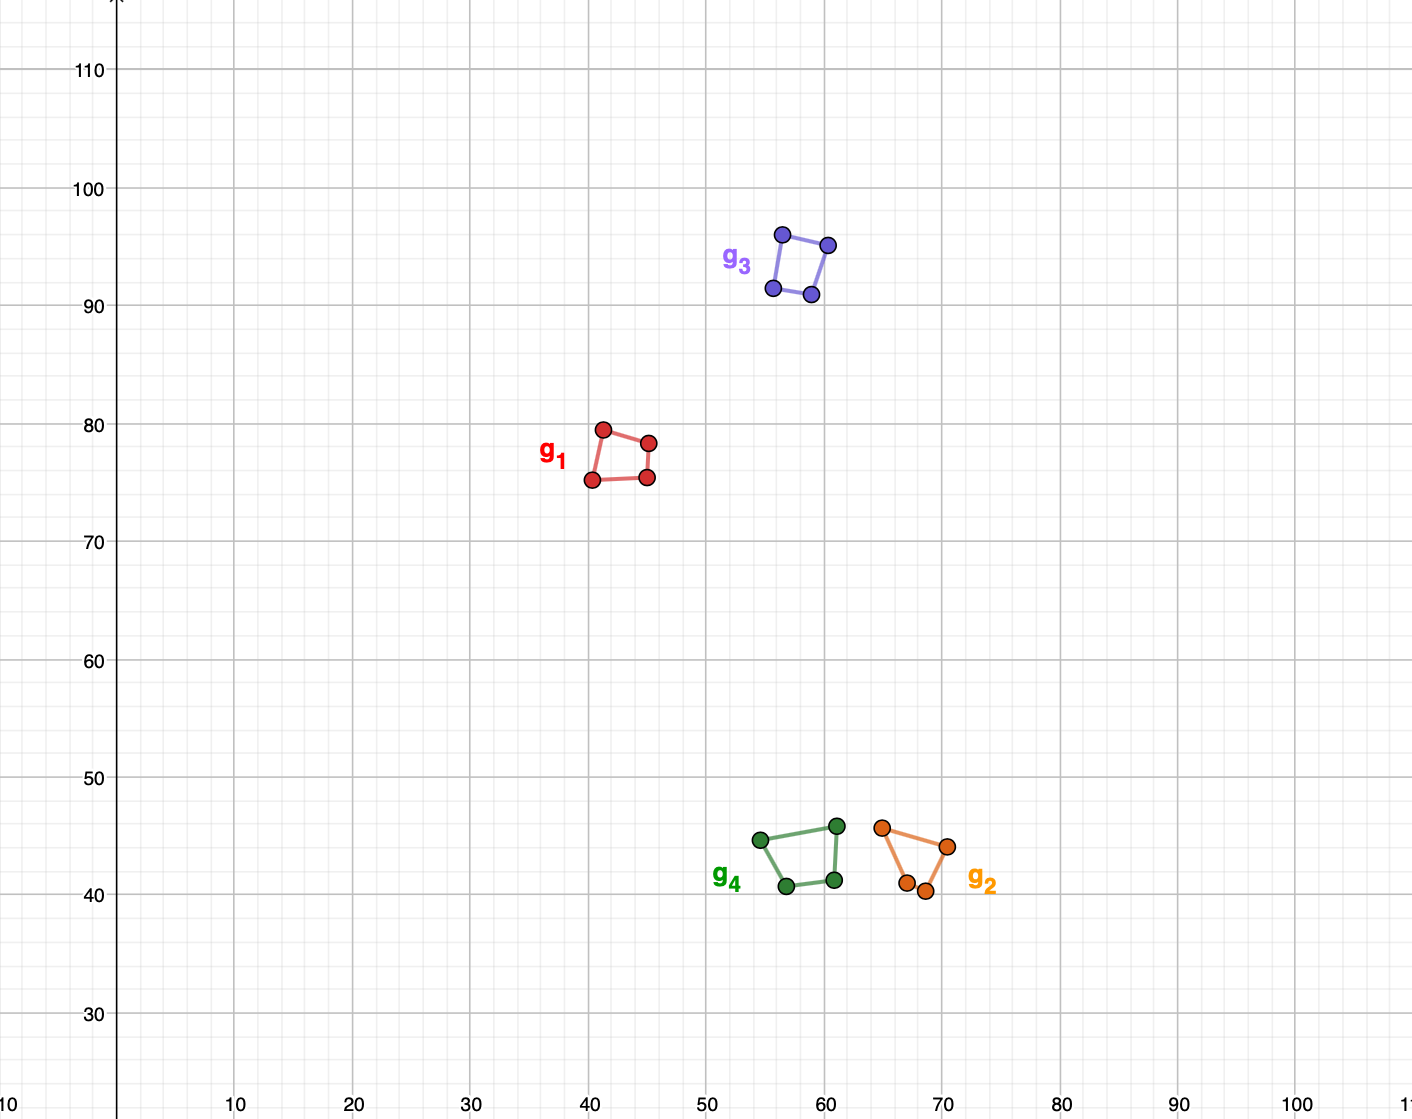
\includegraphics[width = 0.5\linewidth]{figures/example.png}
\caption{Illustrative example \label{fig:example1}}
\end{figure}

\noindent
Figure \ref{fig:example1} shows an illustrative example consisting of four target planar graphs ($g_1$, $g_2$, $g_3$ and $g_4$) to be visited. We assume that their visits must be performed by a fleet of two drones supported by a mothership which starts from the origin $(0,0)$ and ends on the destination point $(100,0)$.



\begin{figure}[h!]
    \centering
    \subfloat[\centering a]{{\includegraphics[width=5cm]{figures/example_tour_g1_Step1.png} }}%
    \qquad
    \subfloat[\centering b]{{\includegraphics[width=5cm]{figures/example_tour_g2_Step1.png} }}%
     \qquad
    \subfloat[\centering c]{{\includegraphics[width=5cm]{figures/example_tour_g3_Step1.png} }}%
    \qquad
    \subfloat[\centering d]{{\includegraphics[width=5cm]{figures/example_tour_g4_Step1.png} }}%
    \caption{STEP 1 for the illustrative example}%
    \label{fig:example2}%
\end{figure}

\noindent
Figure \ref{fig:example2} reports a zoom on each single target graph, showing the tour generated by STEP 1 of the heuristic procedure. A pair of points representing retrieving and launching points,  together with an arrow pointing the direction followed by the drone according with the order in which the edges are visited, are depicted on each edge.

\begin{figure}[h!]
    \centering
    \subfloat[\centering a]{{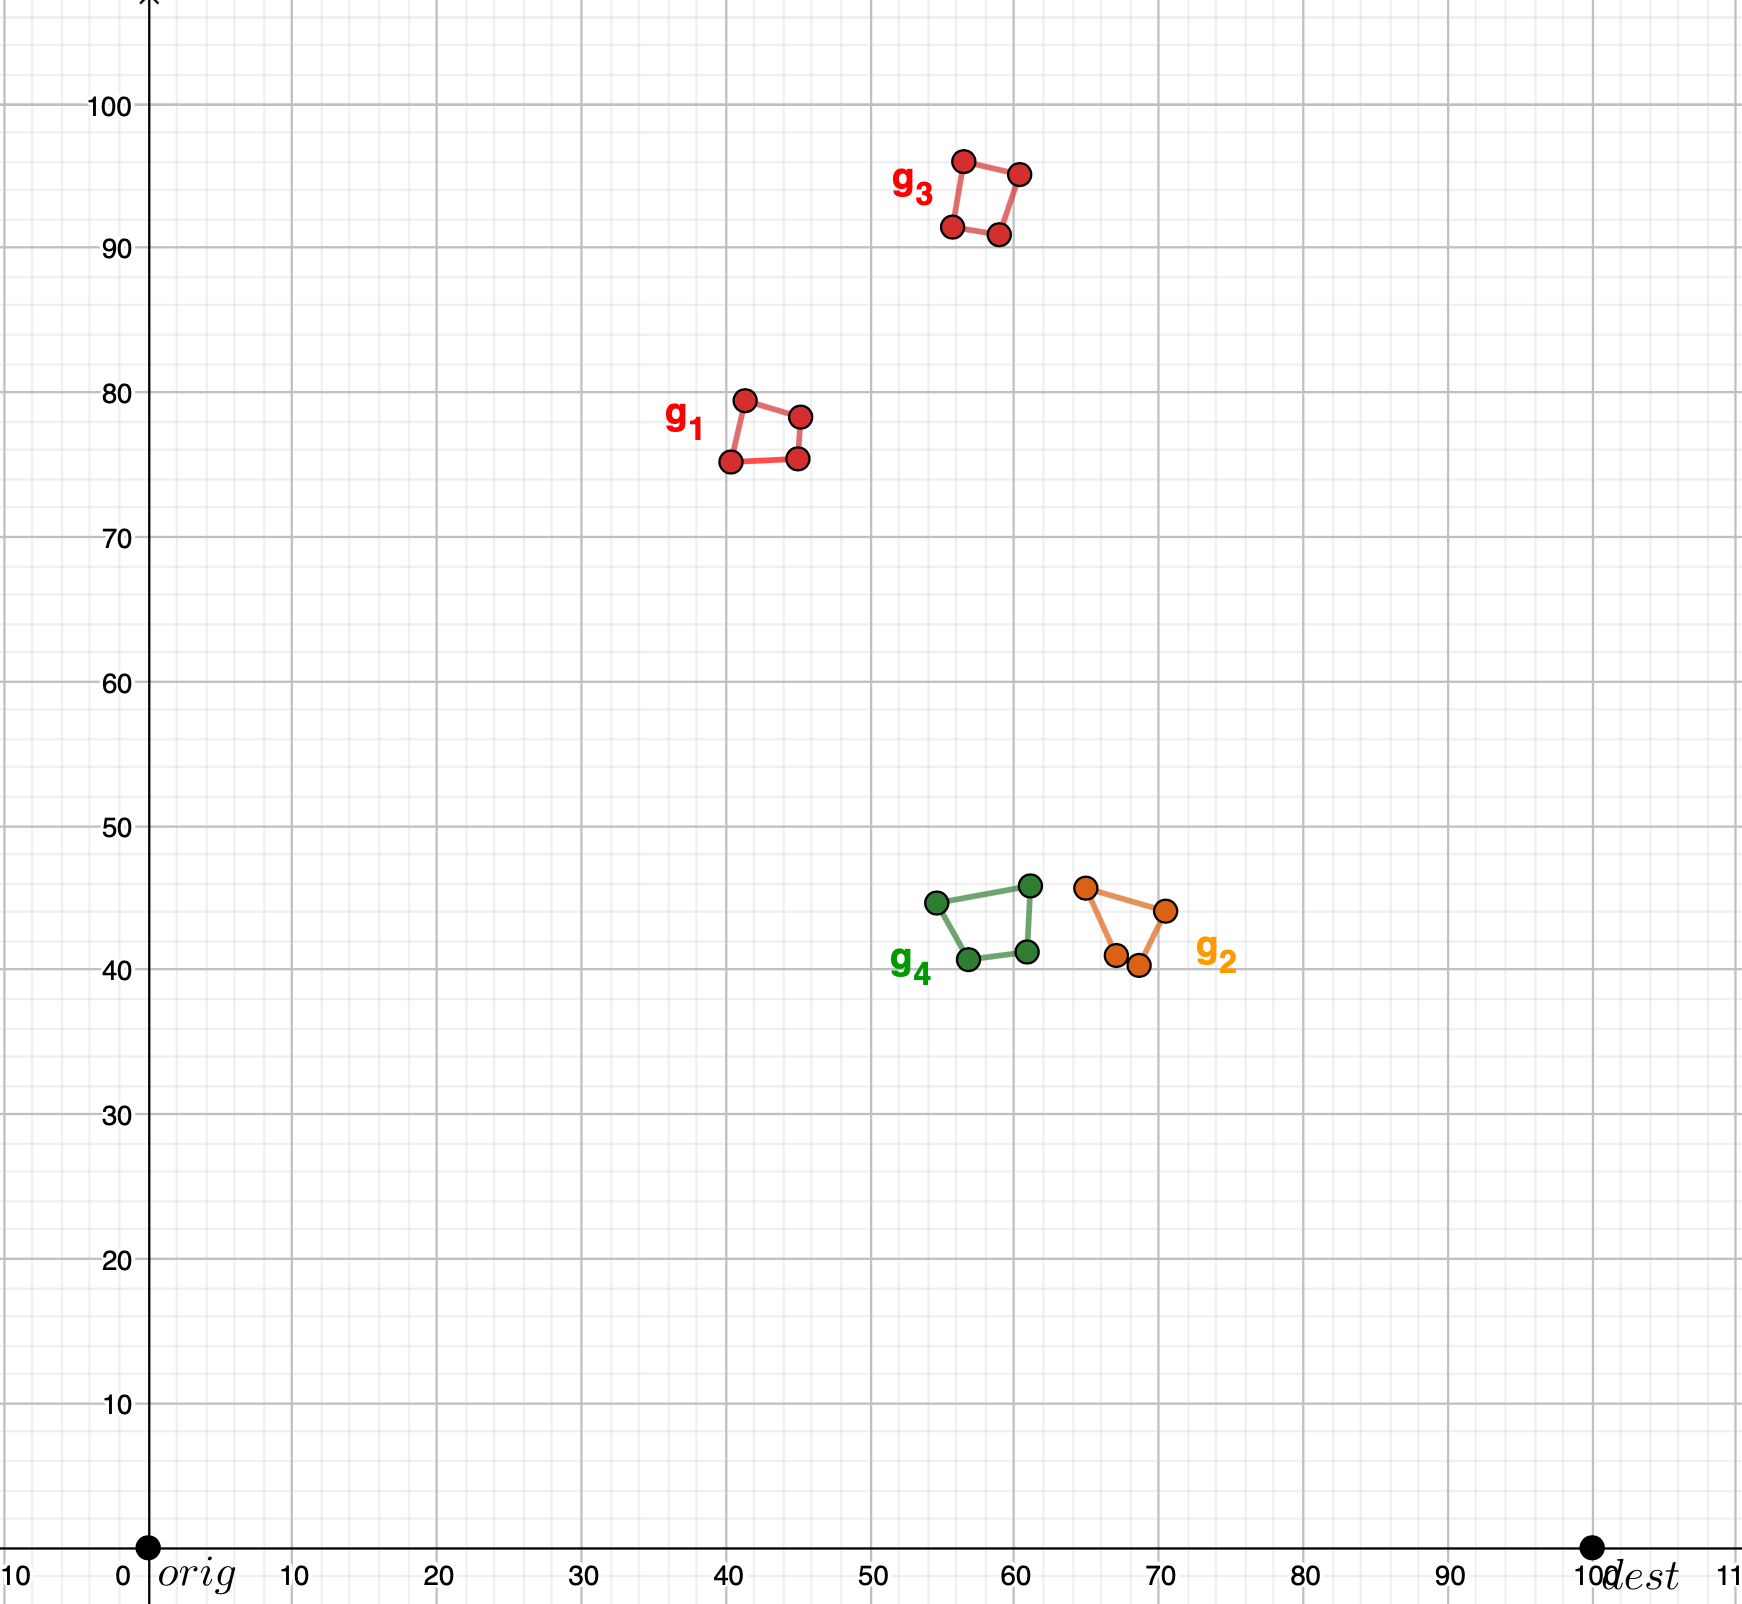
\includegraphics[width=5cm]{figures/example_step_2.png} }}%
    \qquad
    \subfloat[\centering b]{{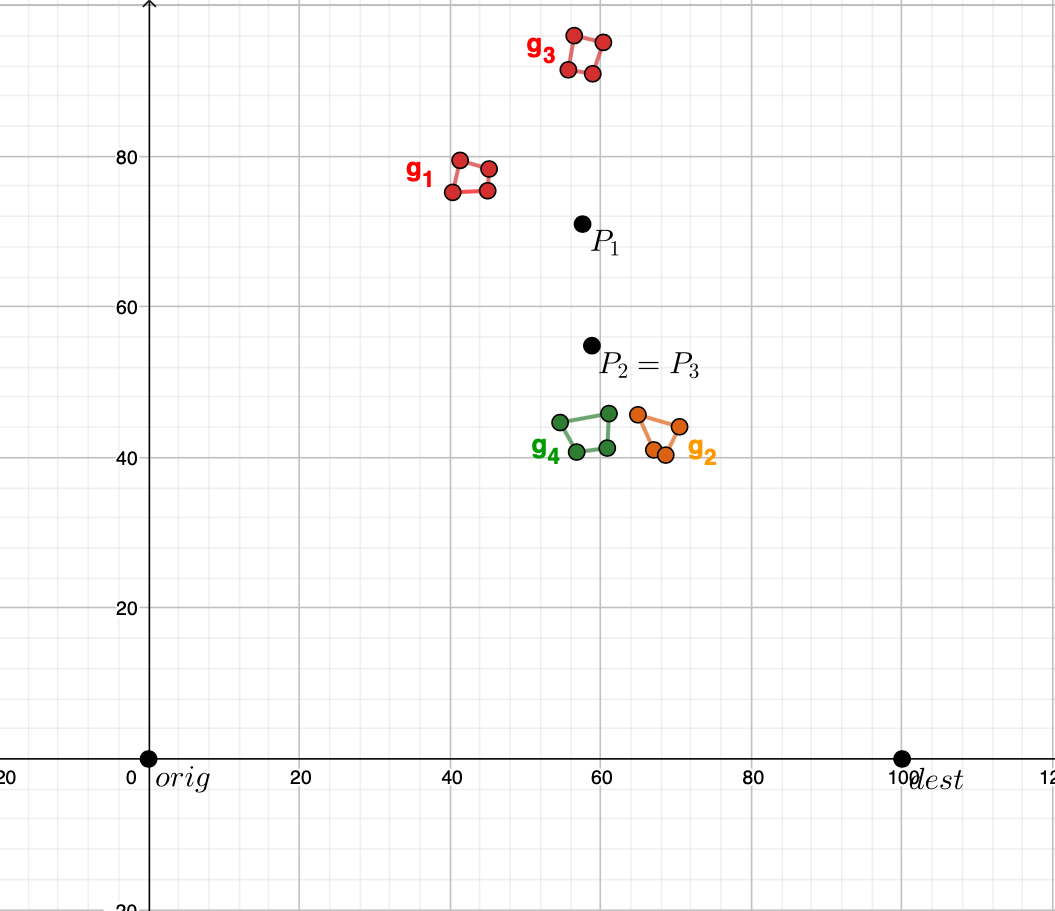
\includegraphics[width=5cm]{figures/example_step_3.png} }}%
        \caption{[a] STEP 2, [b] STEP 3 for the illustrative example}%
    \label{fig:example3}%
\end{figure}

\noindent
By applying STEP 2 to this illustrative example, we obtain three clusters, as shown in Figure \ref{fig:example3}[a]. One cluster contains graphs $g_1$ and $g_3$ (in red), while graph $g_2$ and $g_4$ represent distinct clusters. The computation of the reference points of these clusters, according with STEP 3, produces the points $P_1$ and $P_2 = P_3$, as shown in Figure  \ref{fig:example3}[b]. Note that in this case the reference points for the two clusters containing respectively $g_2$ and $g_4$ coincide, and thus we have only two distinct reference points for the three clusters.

%\JP{*** With 3 clusters we should have three reference points, am I confused? ***}

\begin{figure}[h!]
    \centering
    \subfloat[\centering a]{{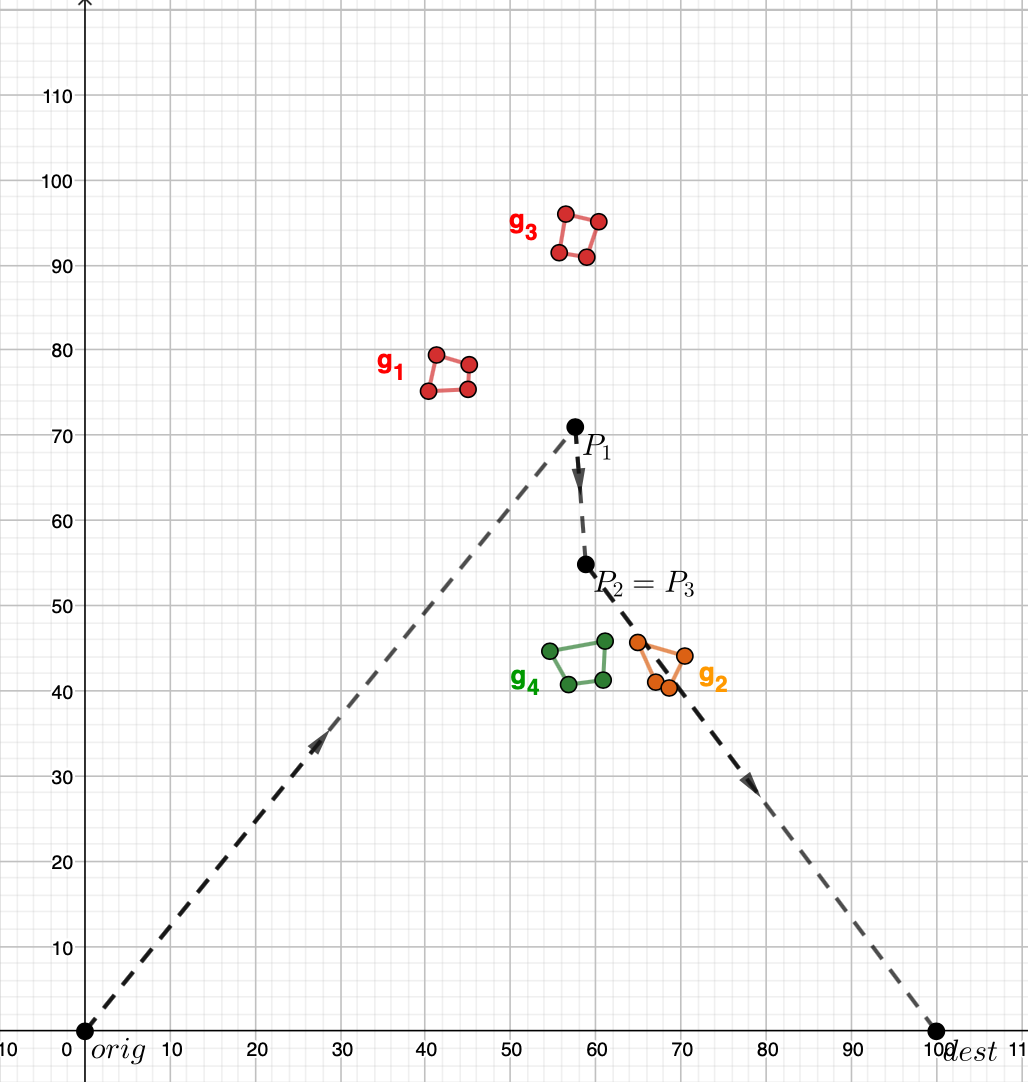
\includegraphics[width=5cm]{figures/example_step_4.png} }}%
    \qquad
    \subfloat[\centering b]{{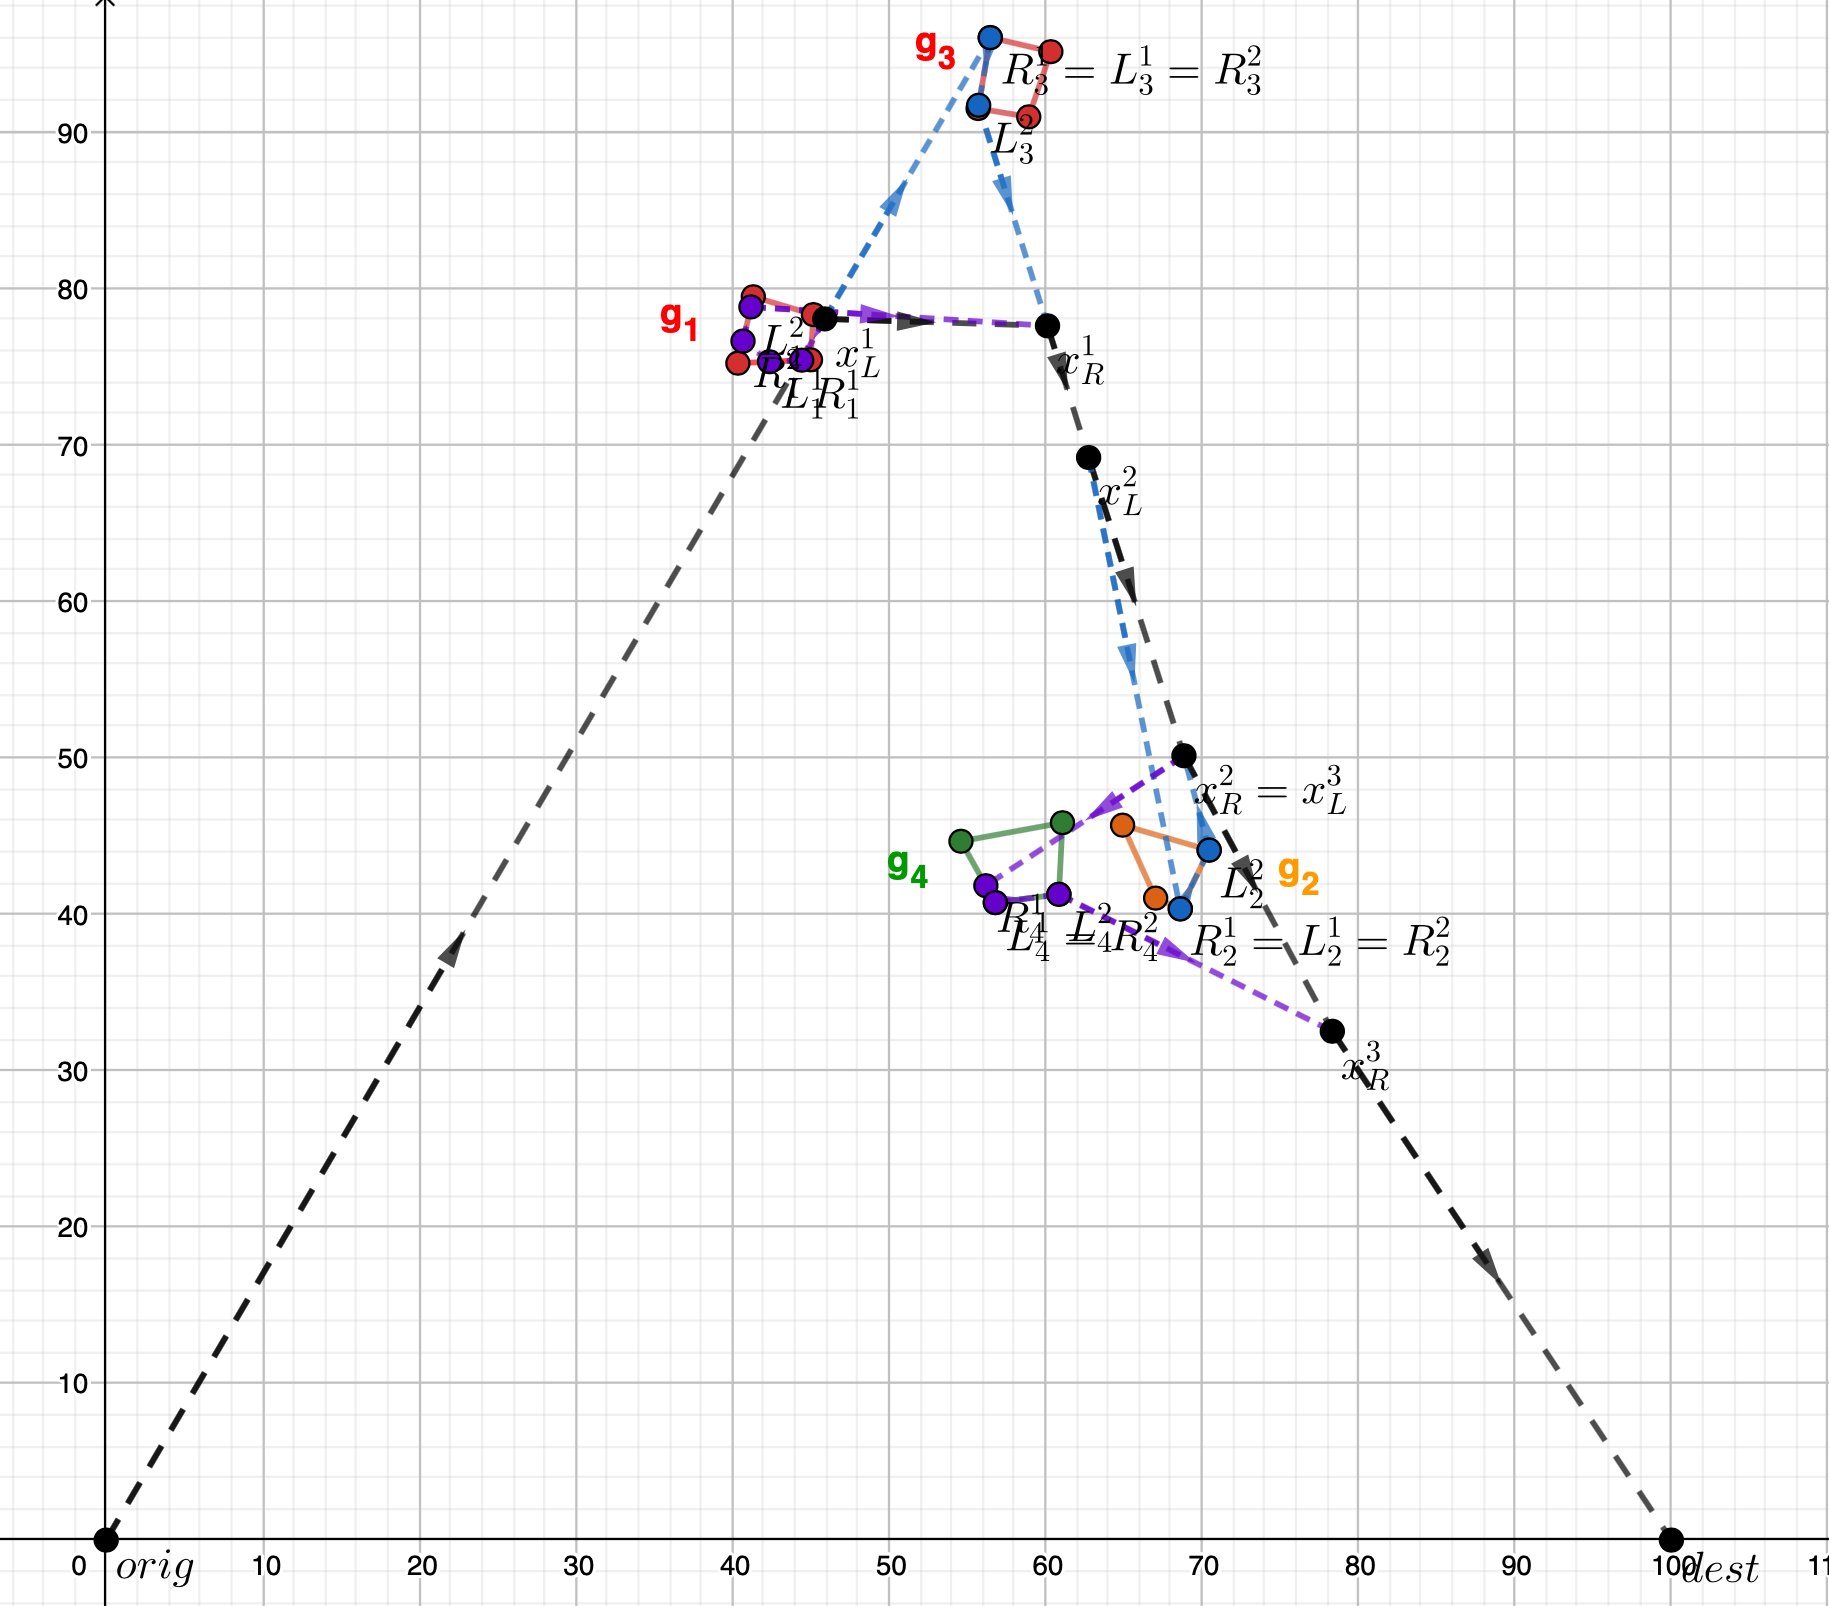
\includegraphics[width=5cm]{figures/example_final.png} }}%
        \caption{[a] STEP 4, [b] STEP 5 for the illustrative example}%
    \label{fig:example4}%
\end{figure}

\noindent
STEP 4 of the heuristic procedure generates the tour of the mothership along the origin point, $P_1$, $P_2$ and the destination point, as shown in Figure \ref{fig:example4}[a]. This tour returns also the order in which the clusters are visited (and thus, also the order of visit to the target graphs) and this permits to set the values of the variables $u^{e_{g}td}$ and $v^{e_{g}td}$ of the \AMD\space model.\\
\noindent 
By providing the initial partial solution obtained by the values of the variables $u^{e_{g}td}$ and $v^{e_{g}td}$, STEP 5 solves the \AMD\space model and returns the final feasible solution shown in Figure \ref{fig:example4}[b]. From it we can observe that the sequence of visit of the target graphs does not change with respect to the one provided by STEP 4. The fleet of two drones first visits graphs $g_1$ and $g_3$ starting from the launching point $x^1_L$. Then, both drones are retrieved by the mothership at point $x^1_R$. The mothership moves to the point $x^2_L$  where one drone is launched for visiting graph $g_2$. Then the mothership reaches point $x^2_R$ to retrieve the drone and from the same point it launches the other drone for visiting graph $g_4$. Then, this drone is retrieved by the mothership at point $x^3_R$ before moving to the final destination point.


\begin{figure}[h!]
    \centering
    \subfloat[\centering a]{{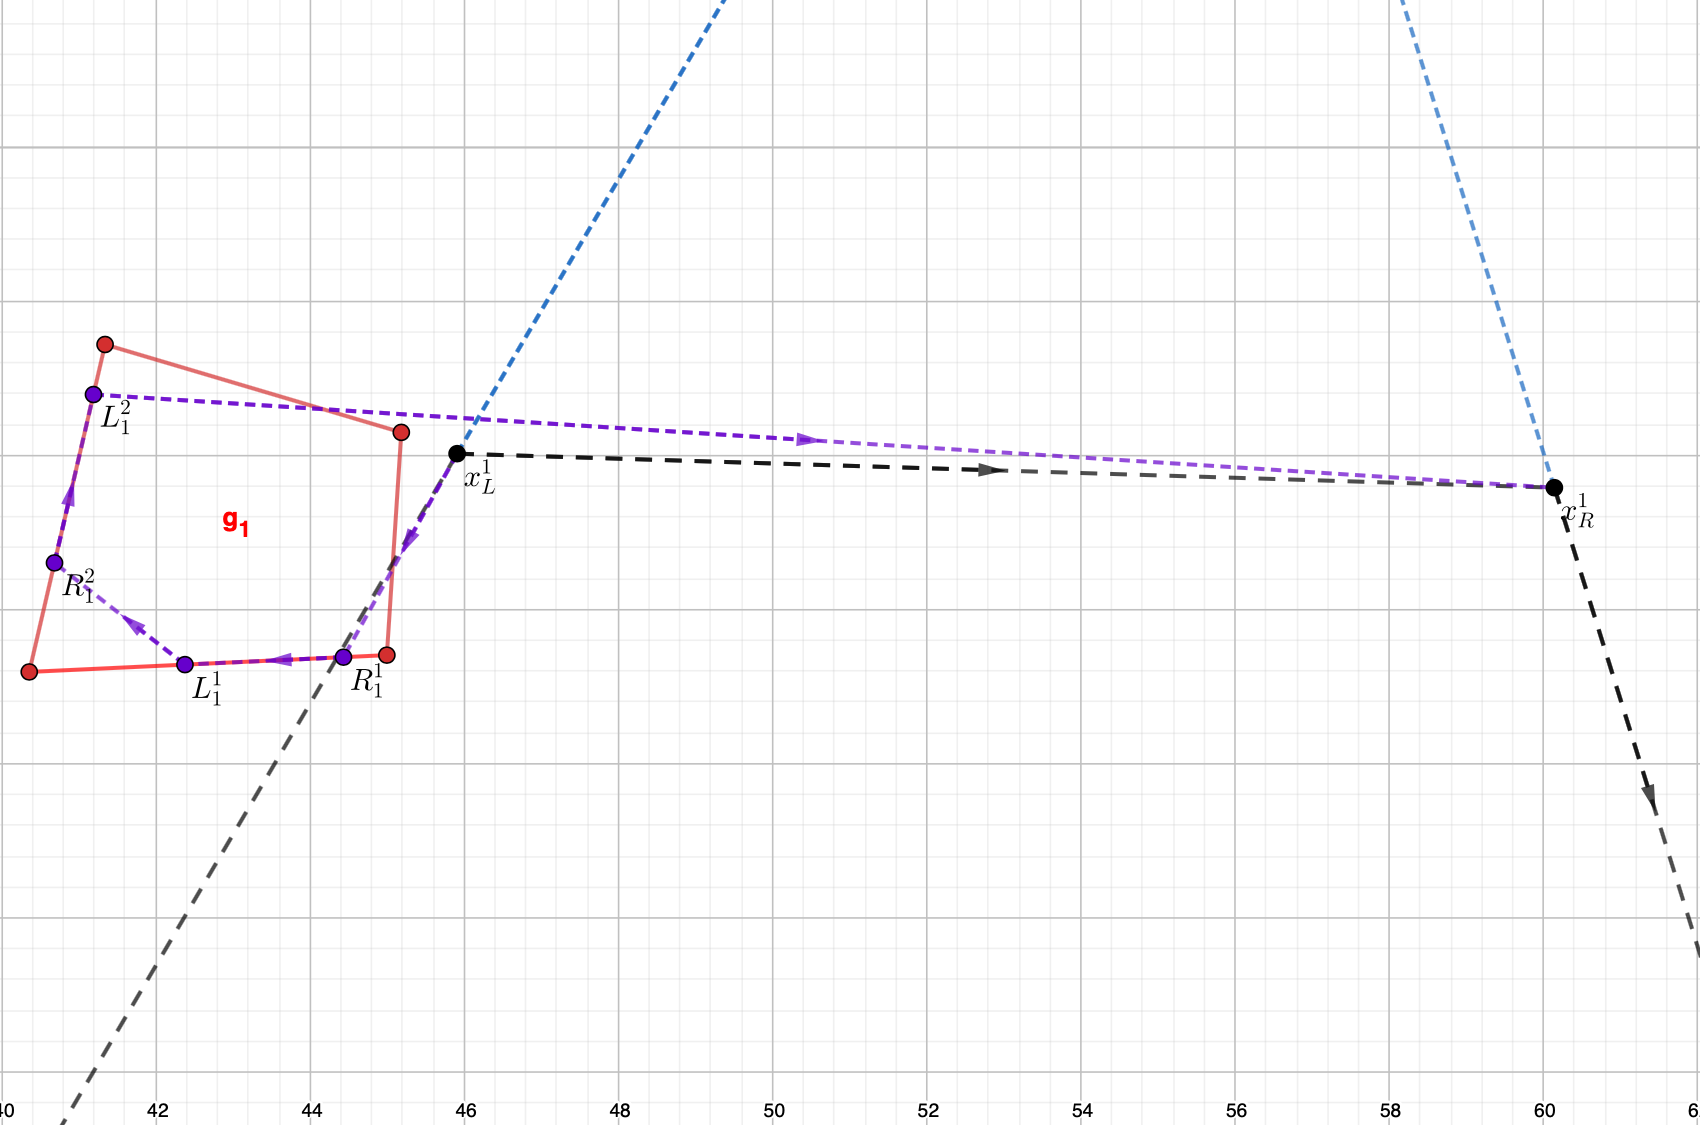
\includegraphics[width=5cm]{figures/example_final-g1.png} }}%
    \qquad
    \subfloat[\centering b]{{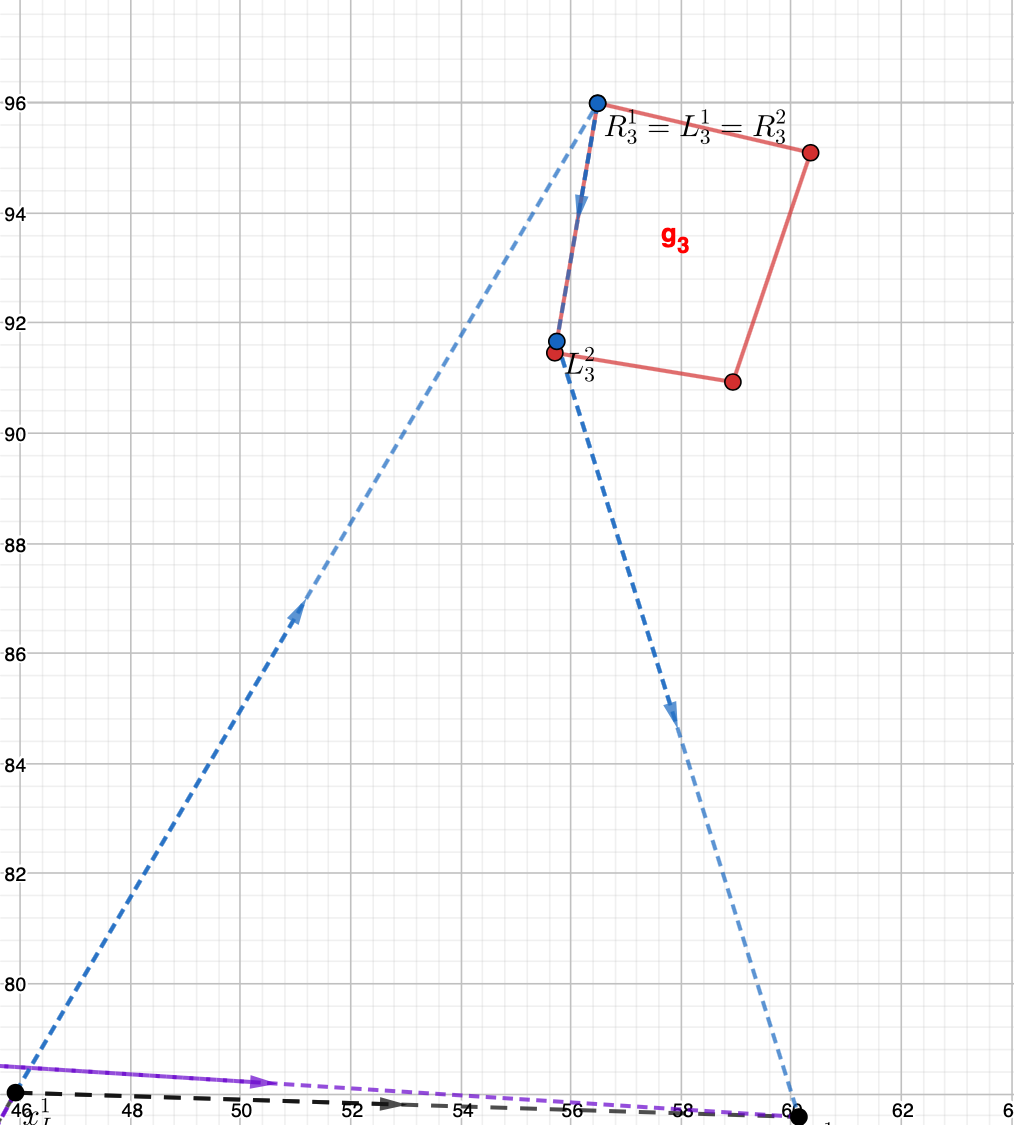
\includegraphics[width=5cm]{figures/example_final-g3.png} }}%
     \qquad
    \subfloat[\centering c]{{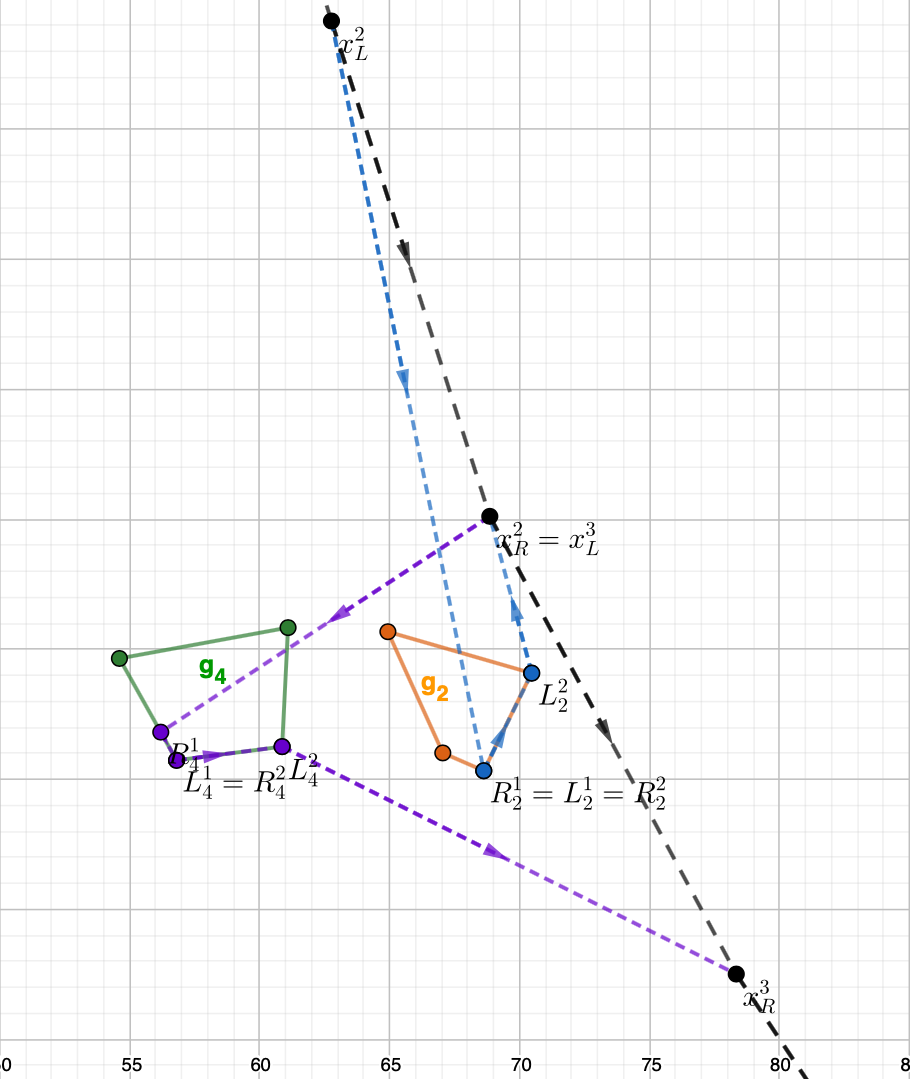
\includegraphics[width=5cm]{figures/example_final-g2_g4.png} }}%
    \caption{Zoom on the tour on each target graph provided by STEP 5}%
    \label{fig:example5}%
\end{figure}

\noindent 
Focusing on each single target graph, Figure \ref{fig:example5} shows the zoom on the tours followed by the drones. For example, Figure \ref{fig:example5}[a] reports the one performed by the drone that visits graph $g_1$. The drone starts from the mothership at point $x^1_L$ and first visits the segment $\overline{R^1_1L^1_1}$. From point $L^1_1$ the drone moves to the second visited edge of graph $g_1$ visiting the segment $\overline{R^2_1L^2_1}$.
Finally, the drone leaves the graph from point $L^2_1$ and it is retrieved by the mothership at point $x^1_R$. Note that in this example the drones do not visit the full 100\% of each graph, but only a pre-specified percentage of each one of them.

\bigskip
\noindent
The reader may notice that the above algorithm can be also used to generate solutions for the model without synchronization  commented in Section \ref{amdasyn} since any solution of the synchronous model is also feasible for the asynchronous one. 

\begin{comment}
\JP{ \textbf{\noindent ***   NOT CLEAR THAT WE SHOULD INCLUDE THIS PART  (JUSTO: dixit) ***}
\bigskip

\noindent
As we already explained in Section \ref{amdasyn}, we also studied a variant of the \AMD\space model in which the mothership can launch and retrieve a drone in different stages. We designed a matheuristic also for this case with similar steps to the one previously presented.
The idea of this procedure is first solving the model with only one available drone (see \cite{art:Amorosi2021}) to determine the optimal launching/rendezvous points associated with each target graph and the corresponding minimum length of the mothership tour.
Then, a clustering procedure, like the one adopted in the matheuristic proposed for the synchronous case, is performed.
After that, the \AMD\space model without synchronization is solved on each cluster setting the launching point of the first cluster equal to the origin. Then the last retrieving point so determined is set as launching point of the next cluster and so on. From the solution obtained for each cluster the total length of the mothership tour is computed as the sum of the partial lengths of each tour associated with each cluster. The same procedure is repeated by starting the clustering procedure with different random seed.\\
In the following, we present the pseudo-code of this algorithm:

\begin{itemize} 
\item[STEP 1] (Launching/rendezvous points)
Solve the AMDRPG model and let $x_L^g$ and $x_R^g \forall g \in \mathcal{G}$ the associated optimal launching/rendezvous points and let $L$ be the associated minimum length of the mothership tour.  
\item[STEP 2] (Clustering procedure)
Initialization: define one cluster for each target graph and set $nit=1$ \\
Select randomly two clusters $C_i$ and $C_j$ (where $i<j$).\\
Check if the number of graphs belonging to the union of $C_i$ and $C_j$ is less than or equal to the number of available drones $n_D$.\\
If this condition is satisfied:\\
search for the point $C$ satisfying the following endurance constraint:
$$
\frac{[d(C, R^{e_g}) + C^{e_{g}e^{'}_{g}} + d(C,L^{e^{'}_{g}})]}{v_D} \leq cap \:\: \forall R^{e_g}, L^{e^{'}_{g}} \in C_i, \:\: C_j
$$
If such a point exists, merge the two clusters and assign to the resulting cluster so obtained the label $C_i$.\\

\item[STEP 3](Launch/rendezvous points exchanges)
Set $i=1$ and $x_L=origin$\\
For each cluster $C_i$ generated at STEP 2:\\
- solve the \AMD\space model with first launching point equal to $x_L$.\\
- let $x_R$ be the last rendezvous point associated with the cluster under analysis, set $x_L = x_R$.\\
Let $L'$ be the associated minimum length of the mothership tour computed as sum of the partial lengths of the tours associated with the clusters.\\
If $L' < L$ update the solution.\\
Set $nit=nit+1$.\\
Repeat STEP 2 and STEP 3 while $nit < maxit$
\end{itemize}
}
\end{comment}


